\graphicspath{{../figures/}}
\begin{abstract}
% P:abstractnew
Can current specialization predict how a shared representation will change with further learning? We construct paired training histories that reach equivalent mean readout measurements but respond differently to a common opposing condition. In the central two-target experiment, the more precisely readable target switches within ten updates in 67.5\% of acquisition-formed checkpoints and 0\% of update-formed checkpoints. Exchanging Adam's second moment reverses the response contrast, including when its mean adaptive scale is held common. Layer and movement controls locate an effect beyond overall update size. Formation records connect small encoder second moments with stronger cancellation between task gradients. A prospective gradient-projection experiment changes this retained state; transferring the resulting second moment alone reduces the ten-update adaptation response in a fixed recipient. The matched comparison extends to three Gaussian targets, while a room-sensor extension retains component effects but fails endpoint matching. Across tested regimes, component effects survive more widely than reversal or reset equivalence. These results identify optimizer-state structure as a causal modifier of adaptation concealed by selected current measurements, with a magnitude and duration that depend on learning conditions.

\end{abstract}

\section{Introduction}
\label{sec:intro}
% P:introquestion
A shared representation supports several prediction tasks, yet limited capacity can make some targets easier to recover than others. We call this inequality in readout precision \emph{representational specialization}. Feature complexity, learning order, and competition between information sources can all produce such biases \citep{lampinen2024biased,pezeshki2021gradient,huang2022modality}. What remains uncertain is whether measuring this specialization also characterizes how readily it will change.

% P:introstakes
This question matters when a model resumes learning after evaluation. Similar current readout quality could coexist with different reallocation of shared features under the same future condition. Training history can affect later plasticity through both weights and optimizer state \citep{achille2019critical,lyle2023plasticity,dohare2024plasticity}. A useful comparison must first separate current measured ability from subsequent response, then intervene on a retained component without changing the recipient weights at the start.

% P:introcontribution
We build this comparison through two routes: observing one target more precisely, or assigning its reconstruction error more weight. After pilot calibration and independent confirmation of selected endpoint measurements, a common opposing condition reveals a large early response difference. We call the difference concealed by those measurements \emph{latent susceptibility}. Component exchanges then show that Adam's second-moment scale and coordinate pattern modify it. Recording and perturbing formation connects this retained state to the gradients that produced it. Finally, changed networks, three targets, and longer continuations distinguish the component effect from the narrower conditions for reversal or reset equivalence.

\section{Relation to training history and optimizer memory}
\label{sec:related}
% P:related1
Similar measured performance can coexist with important differences between predictors, as studied under underspecification \citep{damour2022underspecification}. Representation-similarity measures examine another aspect of their endpoints \citep{kornblith2019similarity}. Our comparison concerns the response to further training: selected reconstruction measurements are matched before a common intervention. This connects the study to plasticity research, where early experience and training dynamics change later learning \citep{achille2019critical,jastrzebski2020breakeven,dohare2024plasticity}.

% P:related2
Optimizer-mediated history effects have direct precedents. \citet{lyle2023plasticity} relates plasticity to loss geometry and shows how unequal adaptation rates of Adam's moment estimates can destabilize training after task changes. \citet{asadi2023resetting} evaluates optimizer resets after changing reinforcement-learning objectives. \citet{ellis2024local} analyzes update-size transients after gradient-scale changes and introduces relative Adam timesteps. These results make inherited adaptive scaling a concrete explanation to test here. Our question is whether average scaling suffices to account for a route difference in \emph{representational reallocation}, or whether the coordinate-wise pattern also changes it.

% P:related3
Direct state transplantation has also been used to study hidden training effects. In a recent preprint, \citet{xu2026optimizer} identifies a first-moment carrier of subliminal transfer: an intervention invisible in immediate outputs produces differences during subsequent training. \citet{sevetlidis2026trainingmemory} organizes historical carriers and proposes state-based causal measurements. The present contribution is a specific empirical decomposition of shared-representation adaptation. It combines matched reconstruction measurements, second-moment scale/pattern interventions, and a common continuation under inherited Adam, fresh Adam, and SGD. Table~\ref{tab:prior} summarizes the closest comparisons.

\begin{table}[t]
\centering\small
\caption{Closest prior comparisons and the question tested here. The interventions and measured outcomes specify how the comparisons relate.}
\label{tab:prior}
\begin{tabularx}{\textwidth}{>{\raggedright\arraybackslash}p{.21\textwidth}>{\raggedright\arraybackslash}X>{\raggedright\arraybackslash}X}
\toprule
Prior work & Established comparison & Present comparison\\
\midrule
\citet{lyle2023plasticity} & Plasticity, loss geometry, and optimizer instability under changing tasks & Reallocation response after matching selected reconstruction measurements\\
\citet{asadi2023resetting,ellis2024local} & Resetting state or time; update-size effects of changed objectives or gradient scales & Component exchange and coordinate pattern at matched mean inverse scaling\\
\citet{xu2026optimizer} & First-moment transplantation and later transfer, including immediate-output invariance & Second-moment structure and the time course of specialization response\\
\bottomrule
\end{tabularx}
\end{table}

\section{Comparing future responses at matched measurements}
\label{sec:design}
\subsection{Two formation routes through one shared bottleneck}
% P:design1
The central learner reconstructs two three-dimensional signals, $A$ and $B$, from noisy observations. We generate standard Gaussian $A$ and independent Gaussian $\epsilon$, and set $B=\rho A+\sqrt{1-\rho^2}\epsilon$ with $\rho=0.35$. A seed-specific orthogonal transformation mixes the observations. A $6\to32\to2$ encoder, with tanh after both layers, maps them to a two-number code shared by two linear reconstruction heads. Training targets are the noise-free signals. This bottleneck makes the allocation of readable information observable.

% P:design2
We manipulate information quality and error weighting separately. \emph{Acquisition precision} changes target-specific input noise before mixing; the high- and low-precision standard deviations are 0.05 and 1.20. Dividing each noisy channel by $\sqrt{1+\sigma^2}$ normalizes its variance. \emph{Update allocation} changes the reconstruction-loss weights:
\begin{equation}
L_t=w_{A,t}\ell_{A,t}+w_{B,t}\ell_{B,t},\qquad w_{A,t}+w_{B,t}=1.
\label{eq:loss}
\end{equation}
Equal weights give the errors equal explicit importance; their gradients can still differ. Observation quality therefore enters learning through a different intervention from changing loss weights. Related work studies active acquisition and task weighting \citep{shim2018joint,chen2022active,chen2018gradnorm,yu2020gradient}; the present design crosses these controls in one shared representation.

% P:design3
After 100 balanced initialization updates, each route runs for 500 updates. Balanced acquisition allocates exactly 250 high-precision updates to each target. For the matched comparison, the acquisition route observes the favored target precisely with equal loss weights; the update route balances acquisition and assigns the favored target weight 0.80. Route strengths are calibrated on pilot seeds and then fixed for confirmation. Appendix~\ref{app:measurement} specifies the measurements and decision rules.

\subsection{Common measurements and paired inference}
% P:design4
To measure readable information, we freeze the encoder, fit fresh linear readouts on unused probe data, and evaluate on separate held-out data. Both targets receive common high-precision inputs. Let $D_A,D_B$ be the variance-normalized mean squared errors. The allocation index
\begin{equation}
s=\frac{D_B-D_A}{D_A+D_B}
\label{eq:s}
\end{equation}
is positive when $A$ is more precisely readable. We align its sign to the originally favored target. A decrease then measures reallocation toward the other target, and crossing zero changes which target is more readable. We also retain both errors, their sum, and allocation under a common low-precision probe. Thus relative advantage is evaluated alongside absolute reconstruction quality.

% P:design5
Each seed supplies a common ancestor and paired input/noise sequences. Conditions branch with the same initial model and, unless manipulated, optimizer state. Pilot and confirmatory seeds are disjoint; each principal comparison uses 40 confirmatory seeds. Mirrored target labels are averaged within seed for inference. We report 95\% seed-bootstrap intervals. Endpoint equivalence requires the interval for the mean paired difference to lie inside each pre-specified margin; it is not an assertion that every pair has identical measurements. All confirmatory seeds are retained. Model parameters and representation geometry may differ after formation.

% P:design7
Before confirmatory runs, each plan fixes the largest acceptable mean differences in allocation-index or normalized-error units. Appendix~\ref{app:measurement} lists these matching tolerances and response margins, together with the separate pilot stages.


\section{Matched specialization conceals a response difference}
\label{sec:latent}
% P:response1
Acquisition alone can select the favored target: with equal loss weights, precise observation of $A$ or $B$ produces mean $s=0.3385$ or $-0.3338$ in 40 independent confirmation seeds (Figure~\ref{fig:headline}a). The two formation routes reach similar measured specializations. All five endpoint criteria pass: aligned $s$, target and non-target errors, total error, and low-precision aligned $s$. The mean aligned-$s$ difference is $-0.0064$ ($[-0.0098,-0.0032]$), inside $\pm0.02$. Mean integrated responses over 200 neutral continuation updates, with balanced observation and equal weights, are also equivalent with either inherited or fresh Adam. Matching therefore covers selected static measurements and one neutral-continuation summary, while leaving response to an opposing condition to be tested.

% P:response2
Each formed learner is copied into three ten-update opposing interventions. An acquisition-only pulse observes the previously less readable target precisely with equal loss weights. An update-only pulse balances acquisition and gives that target weight 0.80. A combined pulse observes it precisely and assigns it weight 0.85. Each pulse is tested with inherited or freshly initialized Adam, keeping the recipient model weights unchanged at the branch point. The response is the decrease in aligned $s$; the route contrast is acquisition-formed minus update-formed decrease.

\begin{figure}[t]
\centering
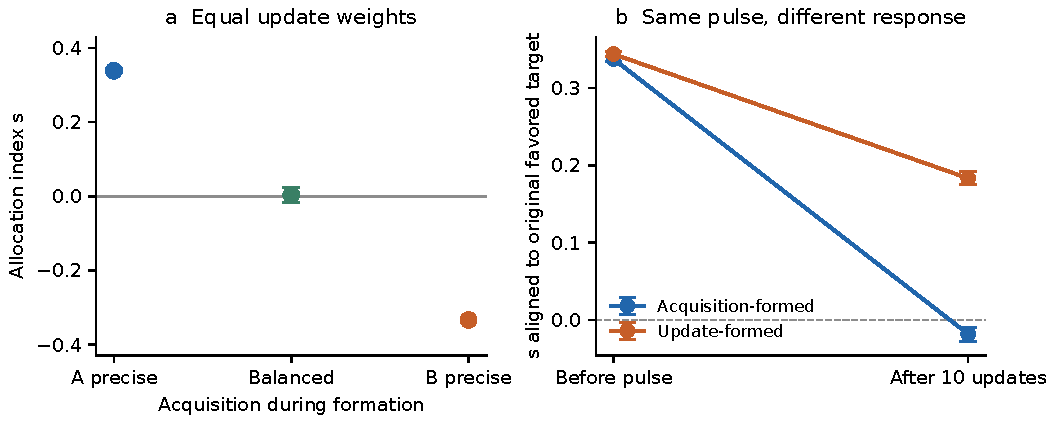
\includegraphics[width=.88\textwidth]{headline_en.pdf}
\caption{A common measured allocation can conceal different adaptation. (a) Acquisition selects specialization with equal loss weights. (b) The matched formation routes receive the same combined opposing pulse. Both move toward the other target, but the acquisition-formed route moves further. Points and intervals summarize 40 seeds; mirrored labels in (b) are averaged within seed. Lines connect endpoints, rather than showing the intervening trajectory.}
\label{fig:headline}
\end{figure}

% P:response3
With inherited Adam, the acquisition-formed route moves further under every pulse (Table~\ref{tab:pulses}). Under the combined pulse, 67.5\% of its checkpoints cross zero within ten updates, compared with 0\% of the update-formed checkpoints (Figure~\ref{fig:headline}b). The continuous route difference is 0.1951. Resetting Adam reduces it to 0.0103, within the pre-specified $\pm0.02$ margin. The other pulses show the same reduction. Thus inherited optimizer state strongly modifies a response difference that selected endpoint measurements and neutral continuation did not reveal.

\begin{table}[t]
\centering\small
\caption{Route difference in specialization lost after ten opposing updates. Brackets give 95\% seed-bootstrap intervals. All inherited-state intervals lie above $+0.05$, and all reset intervals lie inside $\pm0.02$, meeting their respective pre-specified criteria.}
\label{tab:pulses}
\begin{tabular}{lcc}
\toprule
Pulse & Adam inherited & Adam reset\\
\midrule
Acquisition only & $0.1668\ [0.1601,0.1736]$ & $0.0011\ [-0.0010,0.0035]$\\
Update only & $0.1510\ [0.1456,0.1562]$ & $0.0120\ [0.0093,0.0149]$\\
Combined & $0.1951\ [0.1880,0.2021]$ & $0.0103\ [0.0079,0.0129]$\\
\bottomrule
\end{tabular}
\end{table}

% P:response4
This result applies to the two-target network and the ten-update pulses. A separate linear measure of representation similarity (CKA) averages 0.927, and the model parameters are not identical. Resetting Adam leaves those model differences intact. The small reset contrast identifies response equivalence at this ten-update horizon. The zero-crossing rates likewise describe the brief pulse; Section~\ref{sec:time} examines longer common learning.

\section{How retained state changes adaptation}
\label{sec:mechanism}
\subsection{Exchange identifies a second-moment effect}
% P:mechanism1
Adam retains a signed-gradient average $m$ and a squared-gradient average $v$ \citep{kingma2015adam}. The latter sets a separate adaptive scale for each parameter. To test these components directly, we exchange $m$ or $v$ between route endpoints while holding each recipient's weights and optimizer step count fixed. Corresponding parameter coordinates are available because both routes descend from the same ancestor.

% P:mechanism2
In an independent 40-seed comparison, exchanging $m$ leaves the mean response contrast nearly unchanged, with the change inside the pre-specified margin. Exchanging $v$ changes the route contrast from $+0.1968$ to $-0.1265$ (Figure~\ref{fig:moments}a). Both estimates' intervals exclude zero in opposite directions (Appendix~\ref{app:optimizer}). The recipient's second-moment state therefore changes which route is more susceptible. This intervention identifies a causal modifier acting together with the recipient weights and subsequent gradients; it measures the combined ten-update response.

% P:mechanism5
A within-route control holds acquisition, mini-batches, update count, and mean target loss weight fixed. One schedule uses weight 0.80 throughout 500 updates; the other uses 1.00 and 0.60 for 250 updates each in randomized order. The endpoint criteria again pass. The constant schedule then moves further under the common pulse by 0.0324 ($[0.0294,0.0354]$). Exchanging $v$ reverses the contrast to $-0.0141$, while resetting Adam reduces it to 0.0046, inside $\pm0.01$ (Figure~\ref{fig:moments}b). Different acquisition-versus-update labels are therefore unnecessary for this response pattern: equal average loss weights can conceal different optimizer states and later responses. Variability and realized sequence change jointly in this control.

\begin{figure}[t]
\centering
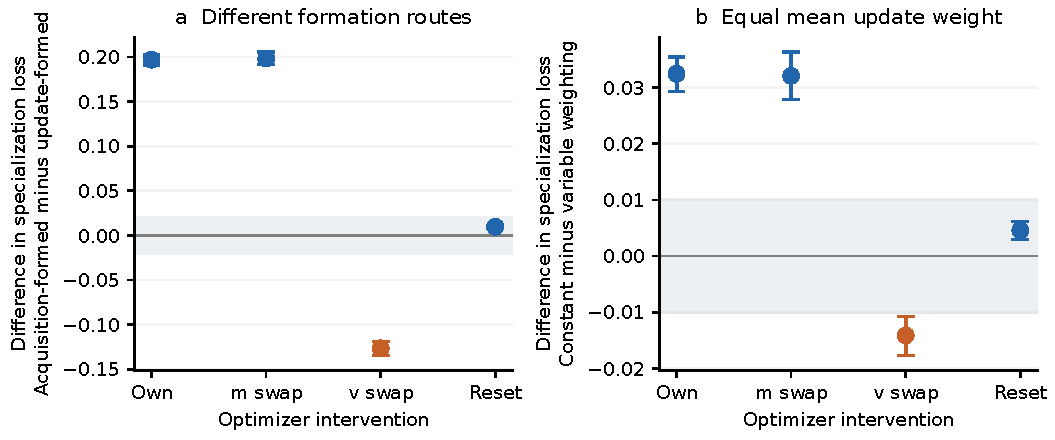
\includegraphics[width=.88\textwidth]{moments_en.pdf}
\caption{Second-moment exchange reverses two short-horizon response contrasts. (a) Acquisition-formed minus update-formed specialization loss. (b) Constant-minus-variable weight-history contrast at fixed acquisition and mean loss weight. Shaded bands show the respective pre-specified equivalence margins ($\pm0.02$, $\pm0.01$). Intervals are paired seed-bootstrap intervals; each comparison uses 40 disjoint confirmatory seeds.}
\label{fig:moments}
\end{figure}

\subsection{Scale, location, and movement}
% P:mechanism3
The exchange raises a more specific question: does one route simply receive a larger average adaptive scale? In a prospective follow-up on 40 new seeds, the inherited-state contrast is 0.1907, reproducing the earlier 0.1951 and 0.1968 estimates. We define $\bar a_v$ as the mean of Adam's bias-corrected inverse-second-moment scaling terms across parameters. This quantity describes the scaling supplied by $v$; an actual update also uses the first moment and current gradient.

% P:mechanism4
Equalizing $\bar a_v$ while preserving each route's coordinate pattern reduces the response difference from 0.1907 to 0.0875. Replacing the pattern by a scalar value gives 0.1251; combining scalarization with a common scale gives 0.0395 (Figure~\ref{fig:timecourse}a). Exchanging the other route's pattern while holding $\bar a_v$ common changes the difference to $-0.0110$. Average scaling thus accounts for part of the response contrast, while coordinate pattern also changes the recipient's response at that common mean. This comparison equalizes a mean inverse-scaling quantity, not the actual update norms throughout the pulse.

% P:mechanism8
A movement-controlled intervention tests whether unequal global path lengths suffice to explain the contrast. At each update, the four branches (two routes, with own or exchanged $v$) receive the geometric mean of their proposed update norms while preserving their directions. With own $v$, the contrast falls from 0.1907 to 0.0303, approximately 84\% under this rule; with exchanged $v$ it is 0.0072, leaving a paired exchange effect of 0.0231. This is a reduction under a different learning rule, rather than the fraction of natural-Adam response causally mediated by movement. The remaining exchange effect shows that equal global movement still permits different reallocation (Table~\ref{tab:ivfmechanism}).

% P:mechanism9
The location of adaptive scaling matters more than its share of total $v$. In acquisition-formed checkpoints, the first encoder layer contains only 5.9\% of total $v$, yet exchanging that layer reduces the contrast from 0.1907 to 0.0115. The heads contain 66.2\%, yet exchanging their $v$ leaves 0.1911. Second-layer exchange leaves 0.0611 (Table~\ref{tab:ivfmechanism}). These interventions retain recipient weights and all other optimizer components. They locate effective interventions in the encoder; their non-additive effects prevent assigning independent causal shares to layers.

\subsection{Formation connects gradient conflict to retained state}
\label{sec:forming}
% P:formationstory
Why is the acquisition route's encoder second moment small? Logging the original 500-update histories reproduces all 160 saved endpoints exactly. The task gradients often point in opposing directions: their negative interaction cancels 94\% and 93\% of the accumulated weighted individual-square sums in the two encoder layers, versus 28\% and 25\% in the update route. The individual-square sums themselves are larger under acquisition. The small second moment therefore reflects cancellation as well as a substantial remaining contribution from the balanced ancestor. This accounting follows actual evolving weights and inputs (Appendix~\ref{app:formationlogs}).

% P:projectionmain
We next alter formation using a two-task PCGrad projection on shared-encoder gradients \citep{yu2020gradient}. When the two weighted gradients conflict, each is projected off the opposing direction; head updates remain unchanged in form. A locally fixed protocol uses 40 new seeds and retains the original acquisition and update routes as controls. Projection raises the acquisition encoder's final second-moment sum by a factor of $1.423\;[1.386,1.459]$ and lowers its mean inverse scale to $0.713\;[0.705,0.721]$ of the original. Transplanting only this projected-history $v$ into the original acquisition recipient changes its ten-update response by $-0.0472\;[-0.0489,-0.0455]$ (Figure~\ref{fig:projection}).

% P:projectionmagnitude
Projection shrinks individual gradients while increasing the squared norm of their sum through reduced cancellation, yet final $v$ remains below the update route (Figure~\ref{fig:projection}a). Because magnitude and interaction change together, it does not partition the original state difference into cancellation and observation-quality contributions.

% P:projectioninterpret
The crossed transplant fixes each recipient while changing $v$: both respond less to projected-history $v$ at ten updates. Projection also changes weights and $m$, and fails endpoint matching. Its total effect therefore supplies neither a matched-endpoint replication nor a natural mediation fraction. It establishes that changing formation produces a different $v$ that alone changes a fixed recipient's response. At 50 updates the donor effects are small and positive. Appendix~\ref{app:projection} gives the factorial comparison, failed criteria and secondary horizon.

\begin{figure}[t]\centering
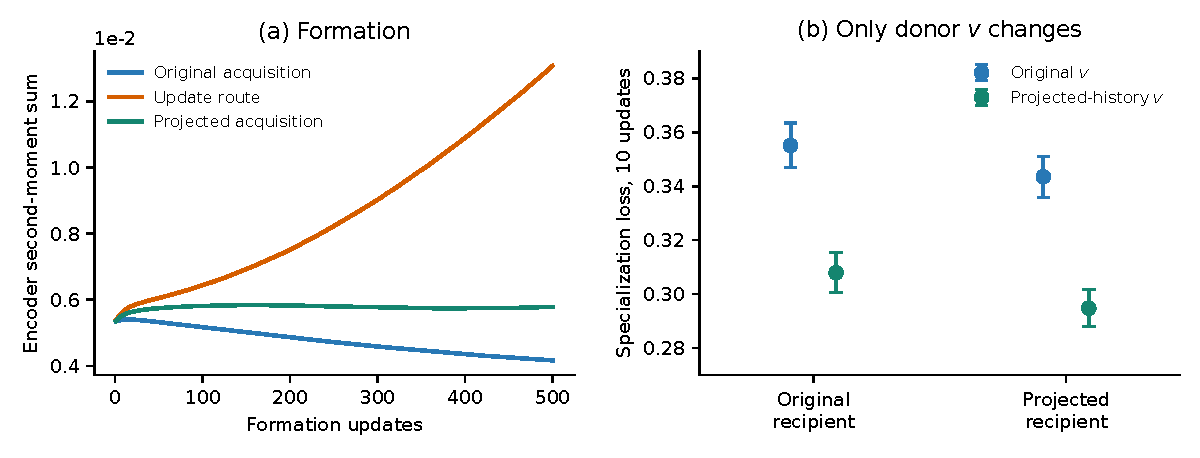
\includegraphics[width=.94\textwidth]{../figures/projection_en.pdf}
\caption{Formation intervention and a fixed-recipient test. (a) Mean encoder second-moment sum during formation in 40 new seeds. (b) Ten-update specialization loss for the two acquisition recipients with original or projected-history second moments. Within each recipient, weights, first moment, and step count are fixed before the pulse; only $v$ changes. Error bars are paired seed-bootstrap 95\% intervals.}
\label{fig:projection}
\end{figure}

\section{The effect has a time scale and a limited scope}
\label{sec:time}
% P:time1
A small difference immediately after reset could still grow during continued learning. We therefore extend the opposing intervention to 500 updates under inherited Adam, fresh Adam, or momentum-free SGD. SGD's common learning rate is calibrated within each seed and target direction using first-batch inherited-Adam update norms and gradient norms, then held fixed; allocation responses are not used for calibration. All three continuations start from the Adam-formed route endpoints.

% P:time2
Inherited Adam produces its largest route differences after 10--20 updates. Fresh Adam gives 0.0096 at update 10 but 0.0274 at update 50; calibrated SGD gives 0.0123 at update 10, 0.0433 at update 50, and 0.0309 at update 100 (Figure~\ref{fig:timecourse}b). The update-50 intervals for fresh Adam and SGD lie above 0.02. That margin was fixed for the ten-update test and is only a reference for later points. The observations show delayed route differences after inherited Adam state has been removed, implicating differences retained on the model side without identifying their specific parameter or geometric source.

% P:time3
The route contrasts shrink toward zero by update 500. Under inherited Adam, the endpoint allocation difference is $-0.00045$ ($[-0.00146,0.00057]$). This endpoint difference is distinct from the difference in change since formation, because the starting measurements were close rather than identical. The inherited-minus-fresh response contrast also changes sign by update 50, so the inherited trajectory is not described by adding a fixed nonnegative fast component to the fresh-Adam trajectory. Within this common opposing condition, optimizer state changes the timing and magnitude of reallocation; the large early difference does not imply a persistent allocation gap.

\begin{figure}[t]
\centering
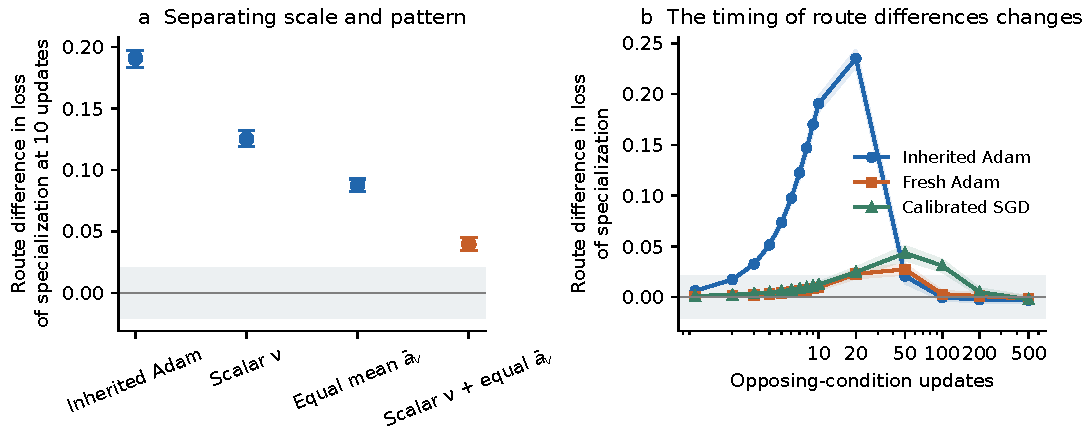
\includegraphics[width=.88\textwidth]{timecourse_en.pdf}
\caption{Scale/pattern interventions and observation horizon resolve different parts of the response. (a) Ten-update route contrast after retaining inherited state, scalarizing $v$, equalizing $\bar a_v$, or both. (b) Continued common opposition under inherited Adam, fresh Adam, or calibrated SGD. The band at $\pm0.02$ refers to the ten-update equivalence margin; later points have no pre-specified decision rule at that margin. Means and 95\% paired seed-bootstrap intervals use 40 new seeds.}
\label{fig:timecourse}
\end{figure}

% P:generalization
Extension IV-F tests the comparison on 32 new paired seeds under changes in hidden width, activation, target correlation, second-moment decay, and formation duration. All nine distinct settings meet the five endpoint tolerances and show a positive common-scale pattern effect (Table~\ref{tab:claims}). This effect subtracts the swapped-pattern route contrast from the own-pattern contrast at the common $\bar a_v$. Reversal and reset equivalence hold in fewer settings. For example, width 64 retains reversal but leaves a reset interval wholly above 0.02. The component effect therefore transfers more broadly than either stronger response pattern.

% P:durationnew
Longer formation does not produce one universal scaling trend. At every tested $\beta_2$, own-state contrasts are larger after 1,500 than 500 updates, and every 1,500-update reset interval exceeds 0.02. At $\beta_2=0.9$, reset increases the contrast at both durations: inherited state can attenuate a route difference. Saved checkpoints show that the acquisition/update mean-inverse-scale ratio grows with duration at 0.999 but falls at 0.9 and 0.99. The 500-update cancellation mechanism thus does not explain the full grid through a uniformly widening scale ratio (Appendix~\ref{app:extension}).

% P:vbmain
Does the component effect depend on having only one alternative target? We form acquisition- and update-driven histories for three symmetric Gaussian targets and test all six ordered changes of favored target. Eight pilot seeds calibrate endpoint measurements without observing adaptation; 40 new seeds test bottleneck dimensions two and three. The response is the decrease in the pairwise allocation index for the original and destination targets, retaining all three reconstruction errors. Both capacities meet all eight mean endpoint criteria. Exchanging $v$ reverses the ten-update route contrast, and exchanging its pattern at a common $\bar a_v$ changes the contrast at both capacities (Tables~\ref{tab:claims} and~\ref{tab:vb}). Reset equivalence holds at dimension two; at dimension three its interval crosses the $+0.02$ boundary and remains unresolved (Appendix~\ref{app:threeadapt}).

% P:naturalnew
The room-sensor extension tests unequal real measurement distributions while retaining the controlled reconstruction task: each room supplies temperature and humidity, so three two-variable targets can replace the Gaussian targets without redesigning the intervention \citep{candanedo2017data,candanedo2017dataset}. Both capacities retain a common-scale pattern effect, but independent confirmation fails endpoint matching (Table~\ref{tab:claims}). This is evidence that the component effect survives this change of input distribution; it is not a matched-endpoint demonstration on natural data. One house and fixed chronological blocks also leave between-building and task generalization untested (Appendix~\ref{app:natural}).

\begin{table}[t]
\centering\small
\caption{Ten-update claims across 13 distinct extension settings. Y: criterion satisfied; N: an interval establishes failure; ?: unresolved. Endpoint matching requires every measurement interval inside its tolerance. Common-scale pattern effect requires a positive interval; reversal requires own positive and exchanged-$v$ negative intervals; reset equivalence requires its interval inside $\pm0.02$. Individual 95\% intervals are used; this inventory is not a success-rate estimate over a population of settings. IV-F has 32 shared seeds; V-B and V-C each have 40, shared across capacities. Baseline occurs only once. Reversal here is a sign criterion; the separate pre-specified requirement that the own-contrast interval exceed $+0.05$ is not met by the two-dimensional room-sensor setting.}
\label{tab:claims}
% P:claimstable
\begin{tabular}{lcccc}
\toprule
Setting & Endpoints & \shortstack{Common-scale\\pattern effect} & Reversal & \shortstack{Reset\\equivalence}\\
\midrule
Baseline ($\beta_2=0.999$, 500) & Y & Y & Y & Y\\
Width 64 & Y & Y & Y & N\\
ReLU & Y & Y & Y & Y\\
$\rho=0$ & Y & Y & Y & Y\\
$\beta_2=0.9$, 500 & Y & Y & N & N\\
$\beta_2=0.99$, 500 & Y & Y & Y & Y\\
$\beta_2=0.9$, 1500 & Y & Y & N & N\\
$\beta_2=0.99$, 1500 & Y & Y & N & N\\
$\beta_2=0.999$, 1500 & Y & Y & Y & N\\
Gaussian, $d_Z=2$ & Y & Y & Y & Y\\
Gaussian, $d_Z=3$ & Y & Y & Y & ?\\
Room sensors, $d_Z=2$ & N & Y & Y & Y\\
Room sensors, $d_Z=3$ & N & Y & ? & Y\\
\bottomrule
\end{tabular}
\end{table}

\section{Implications}
\label{sec:scope}
% P:scope1
The result gives a concrete way to audit continued learning. Measure current specialization, apply the same future learning condition, and test which persistent components alter the response. In this construction, equivalent mean reconstruction measurements coexist with a large early contrast that can be reversed by exchanging $v$. Mean adaptive scale explains only part of that contrast. The equal-mean loss-weight control further shows that average task emphasis can conceal different retained states and responses. Together, these comparisons connect optimizer memory to the reallocation of information within a shared representation.

% P:scope2
A concrete application is evaluating a checkpoint before resuming training on a changed task. The comparison suggests testing a common continuation with optimizer state inherited and reset, alongside current readout quality. In the present system these choices change the timing and magnitude of adaptation. Whether the same diagnostic improves decisions in fine-tuning requires validation on the target task, including its eventual performance.

% P:scopecompact
The matched evidence concerns small bottleneck networks, two or three Gaussian targets, prescribed observation/loss histories, and finite continuation horizons. Matching selected mean readouts does not match all model functions or geometry. The component interventions remain interpretable because they hold each recipient fixed at the branch point; transplantation requires corresponding coordinates from a common ancestor. Testing practical checkpoint choices requires target-task evidence, including final performance, rather than treating faster reallocation as inherently better.

\section{Conclusion}
% P:conclusion
Similar measured specialization can conceal latent susceptibility to further learning in the studied two- and three-target Gaussian systems. Component exchange identifies inherited Adam second moments as a causal modifier of early reallocation, with effects beyond mean adaptive scale and, in the two-target control, beyond global update norm. Formation records and projection-plus-transplant interventions connect the gradient history to a second moment that changes the recipient response. The natural sensor extension retains component effects but fails endpoint matching, separating transfer of the intervention effect from transfer of the concealed-response claim. Reset equivalence and sign reversal depend on capacity, learning conditions, and horizon. Current readout quality, persistent training state, and subsequent learning conditions jointly determine what an adaptation comparison reveals.

\section*{Reproducibility statement}
% P:repro
\ifpublicrelease
Code and generated data are available at \url{https://github.com/culturegeek/matched-specialization-different-adaptation} (\href{https://github.com/culturegeek/matched-specialization-different-adaptation/releases/tag/v1.5.1}{v1.5.1}).
\else
An anonymized code and data archive accompanies this manuscript as supplementary material.
\fi
The archive contains source code, locally frozen plans, seed-level trajectories, checkpoints, and audit scripts for the studies reported here and the wider research program. Code uses MIT; generated data and documentation use CC BY 4.0. The redistributed UCI sensor dataset retains its original CC BY 4.0 attribution. Appendix~\ref{app:status} maps claims to files and gives CPU-based integrity, numerical, figure-generation, and training-reproduction checks.

\section*{Broader impact statement}
% P:impact
The work supplies controlled comparisons for examining shared representations whose input access and learning histories vary over time. Applications to deployed systems require direct validation of the interventions and measurements in those settings.

\section*{AI assistance statement}
% P:ai
Generative AI systems were used extensively to propose most experiment designs and follow-up analyses, implement and execute experiments, analyze outputs, survey literature, and draft and translate the manuscript. The human author initiated the broader research program, commissioned this empirical study, authorized its continuation at major decision points, reviewed the evidence and claims, and accepts responsibility for the paper and its public release.

\bibliography{references}
\bibliographystyle{tmlr}
\FloatBarrier
\appendix
\section*{Guide to the appendices}
% P:appguide
Appendix~\ref{app:optimizer} gives the intervention details and estimates for the central adaptation comparison. Appendices~\ref{app:formation}, \ref{app:maintenance}, and \ref{app:three} examine how specialization forms, what supports it during continued learning, and how formation extends to three targets. Appendices~\ref{app:measurement} and \ref{app:calibration} describe measurement checks and acquisition--compression calibration. Appendix~\ref{app:coordinate} reports failed conditional predictors, while Appendix~\ref{app:factors} reports factor controls, including initial failures and later tests with revised criteria; Appendix~\ref{app:status} distinguishes their statistical status and maps the evidence to reproduction files. Appendix~\ref{app:extension} adds endpoint-prediction checks, fixed-protocol replications, and movement- and layer-controlled interventions.

\section{Endpoint and optimizer contrasts (IV-D--E)}
\label{app:optimizer}
% P:appopt1
IV-D uses 40 confirmatory seeds and two mirrored directions per seed. Mean aligned $s$ is 0.3375 after acquisition-driven formation and 0.3439 after update-driven formation; corresponding target/non-target errors are 0.4034/0.8144 and 0.4000/0.8198. The route strengths are pilot-calibrated, not fitted to the confirmatory endpoints. Neutral-continuation integral differences are $-0.0025$ ($[-0.0064,0.0013]$) with Adam inherited and $-0.0018$ ($[-0.0068,0.0030]$) after reset. Carried-minus-reset response interactions for acquisition, update, and combined pulses are 0.1657, 0.1390, and 0.1848, each exceeding the pre-specified 0.08 criterion.

% P:appmargins
The formation tolerances are $\pm0.02$ for aligned $s$, target and non-target errors, and their sum, and $\pm0.01$ for low-precision aligned $s$. IV-D uses response bands of $\pm0.02$ for neutral continuation and reset responses, and $\pm0.05$ for inherited-state pulses. IV-E uses $\pm0.02$ for the change under $m$ exchange and for the reset response; the within-route update-history control uses $\pm0.01$ for its reset response. These criteria apply to intervals for mean paired differences.

% P:appmarginrule
IV-D classifies a contrast as equivalent when its 95\% interval lies wholly inside the specified band, practically different when it lies wholly beyond either boundary, and unresolved otherwise. All three inherited-state pulse intervals lie wholly above $+0.05$ (Table~\ref{tab:pulses}), indicating positive, practically meaningful route differences. All reset-pulse intervals lie inside $\pm0.02$.

% P:appmarginorigin
IV-D calibrates route strength on pilot seeds 8000--8015 and fixes the tolerances before seeds 8100--8139. IV-E uses pilot seeds 9000--9015 to set response criteria before seeds 9100--9139; the within-route control explicitly uses pilot seeds 9200--9215 to set its response criteria and equivalence margin before seeds 9300--9339. The plans document these operational choices but do not derive the margins from an independent practical-error criterion. Equivalence therefore denotes agreement at the stated resolutions in these synthetic comparisons.

\begin{table}[h]
\centering\small
\caption{Combined-pulse response contrasts under component interventions. IV-E compares acquisition-formed minus update-formed routes; the control compares constant minus variable update-weight histories. Each uses 40 disjoint confirmatory seeds.}
\label{tab:components}
\begin{tabular}{lcc}
\toprule
Component condition & IV-E route contrast & Equal-mean update-history control\\
\midrule
Own state & $0.1968\ [0.1910,0.2029]$ & $0.0324\ [0.0294,0.0354]$\\
Exchange $m$ & $0.1982\ [0.1912,0.2054]$ & $0.0321\ [0.0277,0.0362]$\\
Exchange $v$ & $-0.1265\ [-0.1348,-0.1183]$ & $-0.0141\ [-0.0176,-0.0110]$\\
Reset & $0.0097\ [0.0078,0.0117]$ & $0.0046\ [0.0031,0.0062]$\\
\bottomrule
\end{tabular}
\end{table}

% P:appopt2
In IV-E, the own-minus-$m$-exchange change is $-0.0014$ ($[-0.0044,0.0018]$), inside $\pm0.02$. The acquisition-formed route's total second moment is 0.5577 times the update-formed route's, while the mean coordinate-wise inverse-second-moment scaling factor is 1.950 times larger. This scaling factor is not the actual parameter-update ratio: Adam's update also depends on the first moment, current gradient, and bias correction. Table~\ref{tab:components} gives the main component contrasts.

% P:appopt3
The equal-mean update-history control fixes the target weight mean at 0.80 over 500 updates. Constant-minus-variable endpoint contrasts are aligned $s$: 0.0023 ($[-0.0024,0.0072]$); target error: $-0.0020$ ($[-0.0043,0.0002]$); non-target error: 0.0001 ($[-0.0042,0.0043]$); total error: $-0.0019$ ($[-0.0039,0.0002]$); and low-precision aligned $s$: 0.000756 ($[-0.000532,0.002110]$). The second-moment ratio is 0.8215 ($[0.8140,0.8283]$), and the inverse-scaling ratio is 1.1524 ($[1.1441,1.1615]$). All pre-specified endpoint and response criteria pass. The inference concerns the joint change in weight variability and realized sequence, not an isolated order effect.

% P:appopt4
The prospective follow-up uses 40 new seeds (20000--20039). Adam uses $\eta=0.002$, $\beta_1=0.9$, $\beta_2=0.999$, $\epsilon=10^{-8}$, and weight decay $10^{-5}$. With optimizer step count $t$ and $P$ parameters, define
\begin{equation}
\bar a_v=\frac{1}{P}\sum_{j=1}^{P}\frac{\eta}{\sqrt{v_j/(1-\beta_2^t)}+\epsilon}.
\end{equation}
The acquisition-formed to update-formed ratio is 0.5539 ($[0.5350,0.5732]$) for total $v$ and 1.9042 ($[1.8710,1.9387]$) for $\bar a_v$. These ratios are calculated separately for each seed and target direction, then averaged over directions within seed and over seeds. If $v$ were uniform across coordinates, its total ratio would predict an inverse-scaling ratio of only 1.3513 ($[1.3282,1.3745]$). Exploratory participation ratios, summarizing the effective number of coordinates carrying the second moment, are 19.17 and 38.93, respectively. Total second moment therefore does not reproduce the observed mean inverse scaling; coordinate inequality is associated with the discrepancy.

For common-scale interventions, the geometric mean of the two routes' $\bar a_v$ values is the target $a_\ast$. Pattern-preserving rescaling replaces every coordinate by $c v_j$, where positive $c$ is found by 80 bisection iterations so that $\bar a_v(c)=a_\ast$. Pattern exchange first transplants the donor route's coordinate-wise $v$ into the corresponding coordinates of the recipient model, then applies the same rescaling. Scalarization sets every coordinate to
\begin{equation}
v_j=\left(\frac{\eta}{a_\ast}-\epsilon\right)^2(1-\beta_2^t).
\end{equation}
For scalarization at the recipient's own scale, $a_\ast$ is its own $\bar a_v$ instead of the geometric mean. The recipient model weights, first moment, and step count remain fixed; achieved relative scale error is below $2\times10^{-6}$. These coordinate interventions are defined within models descending from the same checkpoint. Calibrated SGD uses zero momentum and the same weight decay. For each seed and favored target, its common learning rate is the geometric mean across routes of the first-batch inherited-Adam parameter-update norm divided by the current regularized-gradient norm; it then remains fixed (range 0.0194--0.0529, mean 0.03545). Allocation responses are not used in this calibration.

\begin{table}[h]
\centering\small
\caption{Exploratory post-hoc recombination of second-moment mean scale and coordinate pattern. Values are acquisition-formed minus update-formed specialization loss after ten opposing updates, from the fixed follow-up CSVs.}
\label{tab:vdecomp}
\begin{tabular}{lc}
\toprule
Second-moment condition & Route difference $[95\%\ \mathrm{CI}]$\\
\midrule
Own route scale and pattern & $0.1907\ [0.1835,0.1975]$\\
Own scale, scalar pattern & $0.1251\ [0.1187,0.1316]$\\
Common $\bar a_v$, own pattern & $0.0875\ [0.0825,0.0925]$\\
Common $\bar a_v$, scalar pattern & $0.0395\ [0.0342,0.0447]$\\
\bottomrule
\end{tabular}
\end{table}

% P:appopt5
The post-hoc $2\times2$ interaction in Table~\ref{tab:vdecomp} is 0.0176 ($[0.0151,0.0198]$); the corresponding additive reconstruction reaches 90.8\% of the observed mean. These combinations and this statistic were not in the fixed analysis plan, so they do not establish independent additive causes. In the prospective interventions, exchanging the other route's $v$ pattern while equalizing $\bar a_v$ gives a route difference of $-0.0110$. A predictor fitted to the earlier seeds improves prediction of response \emph{differences} on the new seeds, but a response-ratio predictor fails. The $\bar a_v$ ratio contains relative scaling but not the absolute denominator response, so the two findings are compatible.

% P:appopt6
Under continued opposition, route differences in specialization loss at updates 10, 20, 50, 100, 200, and 500 are, respectively: inherited Adam, 0.1907, 0.2353, 0.0207, $-0.0003$, $-0.0023$, $-0.0031$; fresh Adam, 0.0096, 0.0228, 0.0274, 0.0029, 0.0011, $-0.0014$; calibrated momentum-free SGD, 0.0123, 0.0248, 0.0433, 0.0309, 0.0050, $-0.0022$. At update 50, the fresh-Adam interval is $[0.0227,0.0321]$ and the SGD interval is $[0.0368,0.0499]$. At update 500, the endpoint allocation difference is $-0.000454$ ($[-0.001462,0.000568]$), distinct from the drop difference of $-0.003065$ ($[-0.005642,-0.000316]$). In the separate ten-update-pulse-then-neutral trajectory, the allocation-index difference decreases from 0.06197 at update 50 to 0.00984 at update 510. The inherited-minus-fresh difference changes sign by update 50, so a fixed nonnegative fast component added to the fresh-Adam trajectory is inadequate; complete-state convergence remains untested.

% P:appopt7
A post-hoc update-path analysis reads only the fixed follow-up CSVs. Here the two target directions are first averaged within each route and seed; route ratios are then computed within seed and averaged across seeds. All four ratios below use this convention, which differs from averaging direction-specific ratios above. For inherited Adam, the acquisition-formed to update-formed ratios are 1.900 ($[1.867,1.935]$) for $\bar a_v$, 2.028 ($[1.938,2.116]$) for the first parameter displacement, 1.872 ($[1.844,1.902]$) for cumulative ten-update parameter-path length, and 0.987 ($[0.978,0.996]$) for cumulative gradient-norm path length.

% P:appopt8
For seed-level correlations and reconstruction, the $\bar a_v$ ratio averages direction-specific route ratios within each seed, using the convention whose overall mean is 1.9042. The parameter-path ratio instead divides the two route means after averaging target directions within each route and seed. The scaling ratio correlates 0.797 ($[0.644,0.889]$) with parameter-path ratio; the between-route parameter-path difference correlates 0.806 ($[0.681,0.889]$) with the allocation-response difference. Leave-one-seed-out linear reconstruction reduces mean squared error by 28\% using the $\bar a_v$ ratio and 62\% using realized path-length difference. In each fold, both the fitted model and the mean-only baseline use the other 39 seeds.

% P:appopt9
Path length is measured during the intervention, discards direction, and is not manipulated. It therefore describes a candidate mechanism linking scaling to response; quantifying a causal mediated effect requires controlling the realized movement. The reconstruction evaluates the measured ten-update response within these 40 seeds, rather than predicting it from formation endpoints alone.


\section{Formation and redirection controls (IV-A--C)}
\label{sec:controls}
\label{app:formation}
\subsection{Input precision selects specialization under equal loss weights}
% P:controls1
We first ask whether a preference can develop without unequal loss weights. After 100 balanced initialization updates, each checkpoint is cloned into nine formation conditions: three acquisition conditions ($A$ precise, balanced, or $B$ precise) crossed with three update allocations ($0.85/0.15$, $0.50/0.50$, or $0.15/0.85$). Formation lasts 500 updates. Balanced acquisition contains exactly 250 updates with each target observed precisely, in randomized order; every condition receives the same total amount of high-precision information.

% P:controls2
Under equal loss weights, precise acquisition of $A$ yields mean $s=0.3385$, while precise acquisition of $B$ yields $s=-0.3338$. The paired contrast is 0.6723 ($[0.6660,0.6794]$), above the pre-specified 0.30 criterion. Every confirmatory seed favors the precisely acquired target; balanced acquisition remains near zero. Because all conditions are evaluated using common inputs and newly fitted readouts, the difference persists beyond the momentary advantage of seeing a cleaner signal during training. Acquisition precision is sufficient to select specialization under symmetric explicit updating in this system.

% P:controls3
The full factorial explains why this is not a fixed division of labor between information and learning (Figure~\ref{fig:controls}a). Either control can favor a target. Agreement strengthens specialization, while conflict weakens it; at the tested levels, a strong opposing update weight can overcome the acquisition advantage. Both controls act through the gradients of the same network, so distinct interventions need not have orthogonal effects. These are 500-update outcomes, not estimates of limiting equilibria.

\subsection{Acquisition also redirects already formed states}
% P:controls4
Does acquisition matter only before specialization develops? We formed $A$- and $B$-favored checkpoints by asymmetric updating while both targets were observed at noise standard deviation 0.15. We then fixed update weights at $0.50/0.50$ and applied the same three acquisition conditions for 1,000 updates, with neutral checkpoints as an additional reference.

% P:controls5
Opposite-target acquisition changes the favored target in all 40 seeds for both starting states (Figure~\ref{fig:controls}b--d). The terminal $A$-precise minus $B$-precise contrast, averaged across formed states, is 0.7161 ($[0.7108,0.7213]$), close to the neutral-start contrast of 0.7086. Balanced acquisition moves both formed states toward the center. The first zero crossings occur at mean recorded times of 16.9 and 16.8 updates, but trajectories can subsequently move nonmonotonically; these times do not measure settled adaptation. Current acquisition can redirect an update-formed representation under equal subsequent loss weights, within the observed 1,000-update horizon.

\begin{figure}[t]
\centering
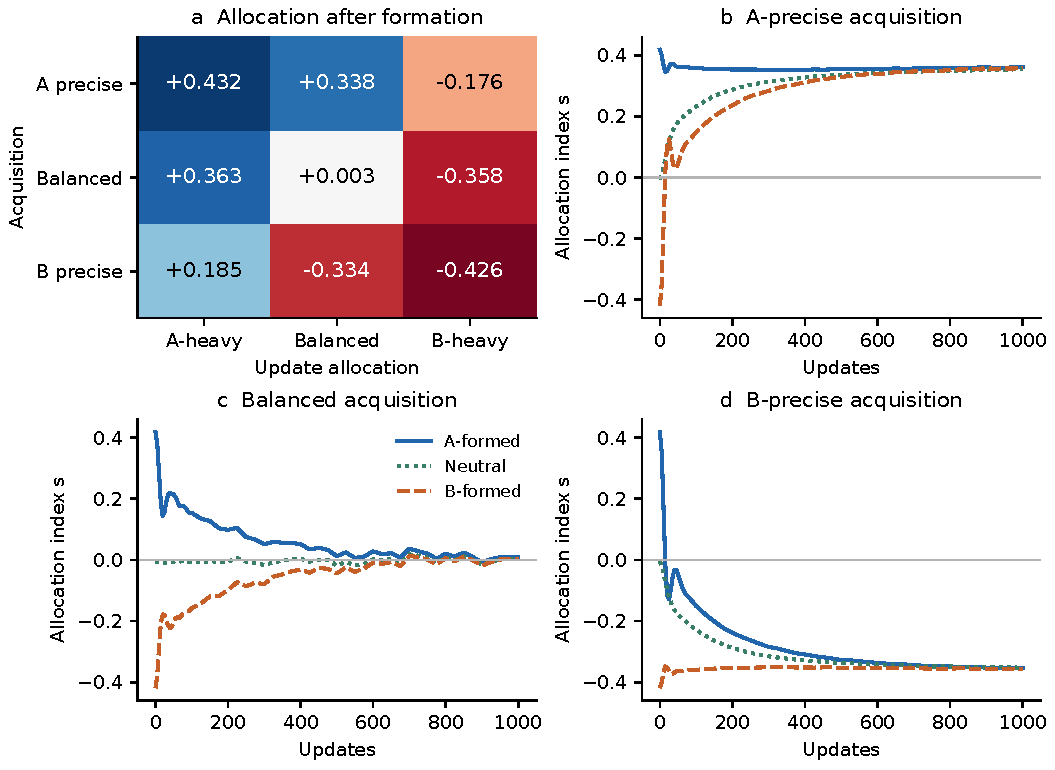
\includegraphics[width=\textwidth]{controls_en.pdf}
\caption{Current acquisition and updating jointly control specialization. (a) Mean allocation after 500 formation updates for the nine acquisition--update combinations. Equal update weights occupy the middle column. (b--d) With all subsequent update weights equal, acquisition redirects previously $A$-formed and $B$-formed states; a neutral starting state supplies a reference. Curves are seed means over 1,000 updates. Their early nonmonotonicity is why first zero crossing is distinguished from sustained switching or convergence.}
\label{fig:controls}
\end{figure}

\subsection{Strong one-sided updating changes the comparison}
% P:controls6
A separate formed-state experiment holds the update target strictly on one side and crosses it with precise acquisition of either the previously favored target or its alternative. Each formed checkpoint is cloned into four conditions for 400 updates. Updating only the reference target retains it as favored in 159/160 cells; updating only the alternative makes that target favored in all cells. Holding alternative-target updating fixed, however, acquiring that target precisely accelerates the trajectory relative to acquiring the reference target precisely. Under a common high-precision probe, the mean first-zero-crossing difference is 3.44 updates ($[2.81,4.00]$). The larger threshold-specific estimate from the pre-specified protocol and its audit remain in Appendix~\ref{app:measurement}.

% P:controls7
Terminal depth also depends on how acquisition and updating combine. In an exploratory analysis, aligned acquisition and update targets yield greater $|s|$ than crossed targets by 0.1411 under the common probe. The acquisition main effect averages to approximately zero because its conditional effects have opposite signs under the two update targets. Thus the data do not support a general rule that acquisition controls only speed and updating controls only direction. Acquisition can select and redirect the favored target; sufficiently strong one-sided updating constrains the outcome while acquisition still changes the trajectory and terminal depth.


\section{Formation, current constraints, and feedback controls (II--III)}
\label{app:maintenance}
\label{sec:maintenance}
\subsection{A formation condition need not remain as a lasting bias}
% P:maintenance1
Once a bias has formed, observing its persistence does not reveal what currently supports it. We therefore remove or change the supporting conditions. In the nonlinear two-target network, making both acquisition precision and update weights symmetric reduces mean $|s|$ from about 0.41 to 0.04 over 400 updates under the common probe. Decay continues through the final observation window. Because both controls are symmetrized, this intervention identifies their joint removal, not the necessity of biased updating alone.

% P:maintenance2
A separate linear bottleneck experiment crosses conditions during formation and continued learning. Its constrained condition combines a one-dimensional representation with one-target updating; its unconstrained condition uses two dimensions and updates both targets. Releasing the formation constraint reduces mean $|s|$ from 0.9706 to 0.1303, above the never-constrained baseline of 0.0592 but far below the formed bias. Further crossings distinguish capacity from update opportunity, as detailed below. Together, these interventions show that a formation history can leave a residual without maintaining its original magnitude under changed current conditions.

\subsection{State-following feedback sustains long-lived regimes}
% P:maintenance3
To test a present sustaining mechanism, a related tanh network receives the complete input while a designed rule chooses which target is updated. The reinforcing rule follows the current allocation index: it preferentially updates the better-represented target. A fixed-propensity control freezes the same rule's probability at its initial value; an exploratory rule favors the worse-represented target. These interventions separate continued tracking of the learned state from an initial tendency to sample one target.

% P:maintenance4
Three tests answer different questions. First, a strong imposed history difference nearly disappears under later common updating. Second, without an explicit history manipulation, state-following feedback amplifies incidental initial differences: terminal $|s|$ is 0.8683, versus 0.4207 under fixed propensity. Third, a separate mirrored-history experiment shows that state following and fixed propensity do not differ detectably in the signed effect of that history, but do differ in absolute specialization depth. The feedback result concerns amplification and support, not a uniquely stronger selection of the history-imposed sign. The detailed estimates below report the separate contrasts.

% P:maintenance5
Capacity changes the maintained specialization. A three-dimensional bottleneck yields almost exclusive readout advantage for one target; a two-dimensional bottleneck yields two regimes with less extreme advantages for opposite targets. Weak opposing update pulses are followed by recovery, whereas stronger pulses can switch regimes. Without externally favoring either target, most trajectories retain their initial regime throughout the 8,000-update comparison. We use ``metastable'' operationally for this finite-time residence, recovery, switching, and coexistence. Counts, longer observations, and hysteresis tests are reported below; the evidence does not establish permanent bistability.

% P:maintenance6
Asymmetric steady states have classical precedent in \citet{harris1997ocular}, while \citet{kiselev2026bifurcation} provides a recent minimal bifurcation construction based on positive feedback. Developmental formation and maintenance have also long been distinguished \citep{crair1998visual}. The contribution here is their intervention-based realization and comparison in learned shared representations. The experiments identify present conditions that sustain a specialization, rather than assigning its persistence to history alone.


\subsection{Detailed estimates}
% P:appmaint1
Experiment II uses a hidden-width-24 tanh encoder and linear heads, with 236 parameters at $d_Z=2$ and 267 at $d_Z=3$. One target is updated per mini-batch. Its principal reinforcement rule is $p_A(s_t)=0.5+\alpha\tanh(\beta s_t)$, with $\alpha=0.40$ and $\beta=1.5$; exploration changes the plus to minus. Balanced updating sets $p_A=0.5$, and initial-fixed updating freezes $p_A(s_0)$.

% P:appmaint2
The history-removal, no-history feedback, and mirrored-history tests are separate. In the first, a strong imposed history difference falls from 1.8822 to 0.0047 under common later learning (residual ratio 0.002); a weak common bias gives ratio 0.003. In the second, confirmatory seeds 300--339 have no imposed initial history: terminal $|s|$ is 0.1817 (balanced), 0.4207 (fixed), 0.8683 (state-following), and 0.0580 (exploratory). The state-following/fixed ratio is 2.064; the paired absolute-difference interval is $[0.368,0.527]$.

% P:appmaint3
In the third test, the first 100 updates use mirrored 55:45 and 45:55 sequences independent of current state. Pooling two disjoint 40-seed cohorts for this exploratory comparison, their immediate signed effect is 0.0811. Terminal signed effects are 0.2240 (fixed), 0.2170 (state-following), and 0.0015 (exploratory); the first two are not distinguishable. Their absolute deviations are 0.4503 and 0.8736, yielding ratio 1.94 and paired difference 0.4233 ($[0.3873,0.4596]$). A mirrored 50:50 order control is consistent with zero. These contrasts support a depth effect without attributing a stronger signed history effect to state following.

% P:appmaint4
The capacity/regime study yields terminal $|s|=0.9842$ with $d_Z=3$ and 0.3902 ($[0.3790,0.4015]$) with $d_Z=2$. Of 80 mirrored arms, 97.5\% lie within 25\% of the median branch magnitude, with 48.7\% on each sign. A separate long run changes $|s|$ by $-0.0004$ ($[-0.0141,0.0134]$) between 8,000 and 16,000 updates. Following 8,000 formation updates, opposite-target forcing for $K=0,800,1600,3200$ gives switching probabilities $0,0.20,0.425,0.65$. Returning and switching trajectories reach 0.985 and 1.015 times the corresponding original/opposite magnitude.

% P:appmaint5
At external update bias $h=0$, positive and negative preparations retain their regimes in 39/40 and 40/40 cases for 8,000 updates. One unforced transition is observed. All 40 bias-sweep seeds switch and return, with mean threshold separation 0.1237 ($[0.1144,0.1337]$). In ten diagnostic seeds, separation decreases from 0.2150 at 500 updates per bias level to 0.1575 at 2,000 and 0.1150 at 8,000. Residence, recovery, switching, and common-condition coexistence define the operational metastability claim; the dwell-time trend prevents inference of a nonzero quasistatic hysteresis width.

% P:appmaint6
The linear constraint-release experiment in III uses independent target signals. With $U$ denoting two dimensions/both targets updated and $C$ one dimension/one target updated, the first letter indicates formation and the second continued measurement-phase learning. Terminal $|s|$ is 0.9862 in UC and 0.9856 in CC. CU falls from 0.9706 at formation to 0.1303, versus 0.0592 in UU. Further separation of the two controls gives 0.9037 for one dimension with both targets updated and 0.3368 for two dimensions with one target updated. This construction differs from the correlated nonlinear network in IV; it supplies a complementary constraint intervention, not another cell of the same factorial.


\section{Three-target formation estimates (V-A)}
\label{app:three}
\label{sec:three}
% P:three1
With two targets, every relative change lies on a single comparison axis. We therefore test the formation result using three symmetric three-dimensional Gaussian targets with pairwise correlation 0.35, mixed into nine input dimensions. The encoder has hidden width 32 and a bottleneck of dimension two or three. Update weights stay at $1/3$. Precise acquisition favors $A$, $B$, or $C$ throughout 600 updates; balanced acquisition allocates exactly 200 precise observations to each target. Each seed branches from the same initialized state. The three-dimensional bottleneck both matches the two-target compression ratio and equals one target's dimension, so it is not a pure control for compression ratio alone.

% P:three2
After formation, the encoder is frozen. Fresh linear readouts are fitted on unused probe samples and tested on separate held-out samples, with common high-precision inputs. We summarize relative errors with centered log-error scores,
\begin{equation}
q_i=\frac{1}{3}\sum_{j\in\{A,B,C\}}\log D_j-\log D_i,\qquad \sum_i q_i=0.
\label{eq:q}
\end{equation}
A positive score indicates more precise readout than the geometric-mean error. Two coordinates describe this observable allocation plane. They are not the coordinates of the full internal representation, and their magnitudes are not directly comparable to the two-target index $s$.

% P:three3
Every target-specific acquisition condition favors its designated target in all 40 confirmatory seeds at both bottleneck dimensions. Relative to balanced acquisition, the designated target's allocation-score gain is approximately 0.37 with a two-dimensional bottleneck and 0.90--0.92 with three dimensions. The effects also spread across the allocation plane (Figure~\ref{fig:three}). To test whether this spread reduces to one empirical comparison axis, we summarize the three mean intervention-effect vectors by singular values. The second singular value measures the component beyond the best-fitting single axis: it is approximately 0.55 and 1.37 at the two capacities, with intervals excluding zero. Near-unit ratios of second to first singular values additionally verify the intended label symmetry. Exact estimates and intervals appear below. Precise acquisition also increases total reconstruction error relative to balanced acquisition: the result is a redistribution of readable information, not a uniform improvement for all targets.

\begin{figure}[t]
\centering
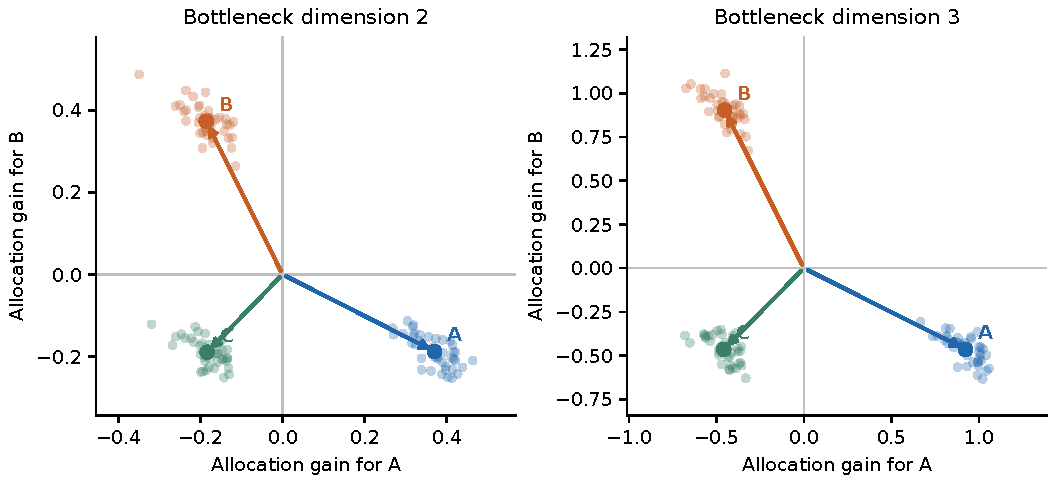
\includegraphics[width=\textwidth]{three_targets_en.pdf}
\caption{Three-target acquisition effects occupy an observable allocation plane. Each point is a seed's target-specific acquisition effect relative to its balanced-acquisition condition, with all update weights equal. Arrows summarize endpoint effects by connecting zero to the mean; trajectories are not shown. The coordinates are gains in $q_A$ and $q_B$, with the change in $q_C$ determined by their zero sum. Both bottleneck dimensions show three label-symmetric, noncollinear effects.}
\label{fig:three}
\end{figure}

% P:three4
This experiment extends acquisition-selected formation to three targets and establishes a second observable contrast. Three-target transitions and optimizer-component exchange remain untested. The result therefore extends the formation claim; testing persistence and latent susceptibility at three targets requires their corresponding interventions.


\subsection{Detailed estimates}
% P:appthree1
V-A uses 40 confirmatory seeds, each cloned across conditions at both capacities. The high-precision acquisition gain is the change in the designated target's centered log-error score relative to balanced acquisition. An update-positive control uses weights $0.8/0.1/0.1$ with balanced acquisition. Table~\ref{tab:three} gives ranges across target labels. All target-specific acquisition conditions favor the designated target in all seeds.

\begin{table}[h]
\centering\small
\caption{Three-target formation after 600 updates. Gain and total-error ranges span the three target labels. Singular values summarize the target-specific intervention-effect matrix; reported values are bootstrap means.}
\label{tab:three}
\begin{tabular}{ccccc}
\toprule
$d_Z$ & Acquisition gain & Update-control gain & $\sigma_2$ & Total-error increase\\
\midrule
2 & 0.3701--0.3731 & 0.4635--0.4668 & 0.5535 & 0.0749--0.0767\\
3 & 0.9030--0.9232 & 1.2239--1.2297 & 1.3656 & 0.1138--0.1148\\
\bottomrule
\end{tabular}
\end{table}

% P:appthree2
The $\sigma_2$ intervals are $[0.5456,0.5612]$ for $d_Z=2$ and $[1.3491,1.3815]$ for $d_Z=3$. The ratios $\sigma_2/\sigma_1$ are 0.9839 ($[0.9725,0.9947]$) and 0.9876 ($[0.9767,0.9971]$), above the pre-specified 0.70 criterion. Nonzero second contrast and near-label symmetry are different claims; neither identifies the dimension of the internal learning state. In an exploratory normalization against the best linear-code distortion floors (0.3344 and 0.0025), acquisition removes 63.23\% and 63.67\% of removable distortion, and the update control removes 75.61\% and 75.39\%. These similarities do not constitute a confirmatory capacity-invariance test.


\section{Network, acquisition, and measurement details (IV)}
\label{app:measurement}
% P:appmeasure1
The central IV network has the structure $6\to32\to2$ with tanh after each encoder layer, followed by linear reconstruction heads. In IV-B, training/probe/test sample counts are 3,072/768/1,536; batch size is 256, learning rate 0.002, weight decay $10^{-5}$, and post-hoc readout ridge coefficient $10^{-3}$. Noisy target channels are divided by $\sqrt{1+\sigma^2}$ before the orthogonal mixing. Training targets are noise-free. IV-B uses 100 initialization and 500 formation updates; IV-C continues formed states for 1,000 updates. These models are nonlinear shared encoders even though their training and post-hoc readout heads are linear.

% P:appmeasure2
IV-A follows 40 seeds with two mirrored formed states through four acquisition--update cells for 400 updates. Under the original probe, crossing the pre-specified aligned threshold $-0.08$ takes 40.6 updates with reference acquisition versus 22.2 with alternative acquisition, holding alternative-target updating fixed. The difference is 18.4 ($[13.2,25.8]$). Remeasuring stored trajectories with common low-noise inputs expands the allocation range from approximately $[-0.154,0.160]$ to $[-0.451,0.462]$. The original-input audit rows are bit-identical to the original trajectories; this is a measurement addition, not a new learning run.

% P:appmeasure3
First-zero-crossing differences are 3.50 under the original probe and 3.44 ($[2.81,4.00]$) under the common probe. Changing the original threshold from 0.04 to 0.06 to 0.08 changes the time difference from 6.50 to 8.44 to 18.38. Thresholds at or above 0.10 increasingly produce non-arrivals and sensitivity to right censoring. The pre-specified 18.4 estimate is therefore threshold-specific; agreement of zero-crossing and continuous-trajectory effects supports the direction of the acquisition effect across measurements.

% P:appmeasure4
The exploratory terminal-depth alignment contrast is 0.0376 with the original probe and 0.1411 ($[0.1370,0.1455]$) with the common probe. The common-probe acquisition main effect is 0.0002 ($[-0.0011,0.0014]$); conditional effects reverse sign, $+0.1413$ under reference updating and $-0.1410$ under alternative updating. Symmetric acquisition/update continuation reduces original-probe $|s|$ from 0.1326 to 0.0146 and common-probe $|s|$ from 0.4067 to 0.0413, with mean residual ratio 0.1009. These outcomes distinguish terminal depth, trajectory, and maintenance rather than assigning all three to an acquisition main effect.

% P:appmeasure5
IV-B's common low-precision probe retains the acquisition contrast at 0.2237. IV-C retains it at 0.2344 ($[0.2322,0.2365]$), compared with the common high-precision formed-start contrast of 0.7161. These cross-probe agreements support the favored-target comparison while demonstrating why allocation-index magnitudes should not be treated as measurement-invariant physical quantities.


\section{Acquisition and compression calibration (Experiment I)}
\label{app:calibration}
% P:appcal1
The acquisition control is calibrated in a linear Gaussian setting where observation loss and compression loss can be distinguished. The decomposition follows indirect source coding \citep{shannon1959coding,wolf1970transmission}. Under squared error, for a target $X$, acquired data $Y$, and a predictor $g(Y)$, conditional-expectation orthogonality gives
\begin{equation}
\mathbb E\|X-g(Y)\|^2=\mathbb E\|X-\mathbb E[X\mid Y]\|^2+
\mathbb E\|\mathbb E[X\mid Y]-g(Y)\|^2.
\end{equation}
The first term cannot be reduced merely by expanding a code constructed from the same $Y$. A representation constraint can further increase the second term.

% P:appcal2
For two correlated three-dimensional targets mixed by a seed-specific random orthogonal transformation, we enumerate channel subsets at observation budgets $B_{\mathrm{obs}}\in\{2,3,4,6\}$ and fit optimal rank-$d_Z$ linear representations for $d_Z\in\{1,\ldots,6\}$. There are 8,192 training and 4,096 test samples per seed, across 20 seeds. The unconstrained mean distortion is 0.0004; acquisition-only and representation-only constraints increase it by 0.3956 and 0.3262, respectively. These are calibration contrasts from the acquisition--representation grid. The best two-channel subsets under the two target weightings have mean Jaccard overlap 0.0167, versus 0.2444 for random subsets. This is a manipulation check for task-dependent acquisition, not an identity forced by the target labels after mixing.

% P:appcal3
A separate analytic check uses a rank-three encoder, for which balanced population error is $D_A=D_B=(1-\rho)/2$. Across six correlations, gradient training with optimal readout matches this curve with RMSE 0.0030 and maximum error 0.0042. Expanding from three to six dimensions improves distortion by 0.3236 in this separate calibration, not the 0.3262 grid contrast.

% P:appcal4
The sequential test supplies four observations, each of $A$ or $B$, giving 16 fixed schedules. A noisy initial cue predicts the later target demand; a cue-dependent policy chooses a complete schedule once, rather than repeatedly tracking an internal learned state. Selection uses 30,000 training and 10,000 validation samples, followed by 20,000 independent test samples. The best fixed objective is 0.181864; the cue-dependent objective is 0.124223, a 31.7\% reduction. Shuffling the cue yields 0.181039 with the same policy class. The gain therefore depends on cue information rather than the larger class alone.

% P:appcal5
Temporal dependence also couples neighboring schedules. If $L_s(W)$ and $L_t(W)$ are endpoint-policy losses, the shared-decoder excess
\begin{equation}
B(\alpha)=\min_W\{(1-\alpha)L_s(W)+\alpha L_t(W)\}
 -(1-\alpha)\min_W L_s(W)-\alpha\min_W L_t(W)
\end{equation}
is nonnegative for $0\leq\alpha\leq1$ by construction. For an interior mixture and attained minima, zero excess requires a common minimizing decoder. The measured result is the frequency with which this common-optimum condition fails: positive excess occurs on 0/32 neighboring paths at temporal correlation $\phi=0$, 4/32 at 0.4, and 18/32 at 0.8. The maximum is 0.039801, and dedicated decoders remove the excess. At $\phi=0.8$, the exact population policy objective has two local optima; 13/20 jointly trained seeds reach the oracle schedule.


\section{A candidate coordinate fails conditional prediction (III)}
\label{app:coordinate}
% P:appcoord1
A separate test asks whether a slowly changing variable predicts switches between maintained specializations. An externally specified loop couples representation, a framing variable $\kappa_t$ that sets task emphasis, and evaluation sensitivity. Eighty arms form history-consistent regimes with mean $|s|=0.9854$. No spontaneous switch occurs in 8,000 unperturbed updates; the 90th-percentile weak-perturbation recovery time is 200 updates, giving an observed time-scale-ratio lower bound of 40. Independent reconfirmation with opposing forcing lasting $K=0,1600,3200,4000,4800,5600,6400$ updates gives rounded switch probabilities $0,0,0.138,0.450,0.688,0.838,0.938$.

% P:appcoord2
The original, disjoint coordinate-audit sample has rates 0.4625, 0.6250, and 0.8750 at $K=4000,4800,5600$. AUC measures how well a predictor ranks switching above non-switching trajectories. The pooled $\kappa$ AUC is 0.712, versus 0.600 for $s$. Within those intervention levels, the $\kappa$ AUCs are 0.565, 0.567, and 0.380. Seed-separated five-fold validation changes AUC by 0.0049 when $\kappa$ is added to $K$ and $s$, while log loss worsens slightly. The two sets of switch rates therefore describe different samples, not conflicting estimates from one CSV. An earlier II head-distance candidate also fails an independent conditional test (AUC 0.373 at $K=1600$). These are failures of the tested predictors, not proofs that no compact dynamical coordinate exists.


\section{Supporting finite-state factor controls (III)}
\label{app:factors}
% P:appfactors1
A separate resource-management environment tests whether task framing, causal prediction, prediction horizon, evaluation horizon, risk sensitivity, and stopping can be manipulated distinctly. A controller supplies current demand from a five-level resource while maintaining equipment against future failure. Resource level, binary demand, and binary equipment state give 20 external states. Standard sensors have accuracy 0.62; an additional target-specific sensor has accuracy 0.94. A ten-step dynamic-programming oracle supplies policy and Pareto references, with a tradeoff environment and a null environment admitting a common optimum.

% P:appfactors2
The initial confirmatory run passes framing and prediction-horizon checks but fails causal-model, evaluation-horizon, and risk-sensitivity criteria. The transition intervention is too small, the evaluation effect misses its threshold, and the risk threshold exceeds baseline risk. Revised strengths and attainable relative criteria are fixed before 40 new seeds, where all five families pass. These later successes do not change the status of the initial failures. A reframing factorial switches only when long prediction, long evaluation, and frame plasticity jointly occur under the designed rule; better alternative information improves frame--equipment agreement rather than simply increasing switch counts. These controls support the infrastructure for manipulating the specified factors separately.


\section{Statistical status and provenance}
\label{app:status}
% P:appstatus1
Confirmatory outcomes retain their pre-specified observation windows, contrasts, and margins. Terminal-depth alignment in IV-A and removable-distortion normalization in V-A are exploratory. Threshold sensitivity and conditional predictor tests are audits, not replacements that retroactively redefine the primary outcomes. Within-seed pairing is preserved; mirrored labels are not independent seeds. Failed initial factor checks and failed conditional predictors remain reported in Appendices~\ref{app:factors} and \ref{app:coordinate}.

% P:appstatus2
The question-based sections map to the reproduction records as follows: formation and redirection use IV-B, IV-C, and IV-A; current support uses II, III's constraint-release construction, and IV-A neutral continuation; latent susceptibility uses IV-D, IV-E, the IV-E update-weight control, and the IV-E follow-up; the conditional coordinate audit uses III-C; three-target formation uses V-A. Experiment I supplies acquisition--compression calibration. The follow-up's fixed intervention tests and its later post-hoc recombination are stored and labeled separately. The constructions provide complementary tests under their separately specified parameters.

% P:appstatus3
The archive's \texttt{docs/PAPER\_TO\_DATA.md} links each figure and principal table to its input files. From the archive root, \texttt{python scripts/verify\_data.py} checks preserved-file hashes and the follow-up's frozen plans and results; \texttt{python scripts/check\_core\_results.py} independently recomputes 27 central means from stored CSVs. After installing \texttt{requirements-analysis.txt}, \texttt{python scripts/make\_figures.py} regenerates the five English figure families. The numerical check covers the selected means. A separate interval ledger links every printed confidence interval to a saved result and its rounding precision. The pooled mirrored-history depth contrast and the two IV-A terminal-depth contrasts use 20,000 paired seed-bootstrap resamples, with mirrored labels averaged within seed. Their reproducible exploratory calculations are provided by \texttt{scripts/audit\_manuscript\_intervals.py}; registered experiment results and decision criteria remain separately identified.

% P:appstatus4
Training reruns are described in \texttt{docs/REPRODUCING.md}, including a one-seed trajectory comparison and the full 40-seed follow-up. The recorded follow-up environment is Python 3.11.7, NumPy 2.4.6, and PyTorch 2.13.0 on CPU with one thread. The environment and scope of the separate package checks are recorded in \texttt{provenance/validation.json}; they do not constitute a rerun of every historical experiment. Reruns write to new output directories so that the archived confirmatory data, failed criteria, and exploratory records remain available for comparison.

% P:appfprovenance
The IV-F files are in \texttt{experiments/iv-extension/}. The two registration files record local pre-run hashes. Its \texttt{README.md} maps all modes, predictions, layer summaries, and failed criteria to data and rerun commands. \texttt{audit\_extension.py} independently checks raw-CSV means, completeness, shared starts, norm constraints, and frozen hashes. Before new training, the baseline checkpoint and six pulse modes reproduced saved seed 20000 exactly.

\section{Endpoint prediction, transfer, and mechanism extensions (IV-F)}
\label{app:extension}
% P:appfintro
The extension asks which parts of the short response contrast are predictable from saved endpoints, transfer to altered networks and targets, and survive control of movement. Existing-data analyses use three disjoint 40-seed cohorts. New training uses the same 32 previously unused seeds (32000--32031) across nine settings, comprising four architectural/target settings and a $3\times2$ second-moment-decay/formation-duration grid with one shared baseline. Layer and movement interventions reuse 40 saved follow-up seed pairs. The protocol and code were locally frozen before these new runs; the existing-data analyses remain exploratory. Mirrored directions are averaged within seed. Intervals use 5,000 paired seed-bootstrap resamples and are individual 95\% intervals.

\subsection{Do residual endpoint differences predict the response?}
% P:appfpred
Within each cohort, we predict the combined-pulse response contrast from the paired endpoint differences in target error, other-target error, and low-precision aligned $s$. Ordinary least squares uses training-fold standardization and a held-out-seed evaluation. Its baseline predicts the mean of the other 39 seeds. Error ratios near or above one indicate little predictive benefit (Table~\ref{tab:ivfendpoint}). Applying the IV-D coefficients unchanged to IV-E and the follow-up gives error ratios 1.032 and 0.999 relative to the IV-D mean predictor. The intercept estimates the contrast at zero differences in the three measured features; it is a conditional linear description, not a causal adjustment for unmeasured geometry.

\begin{table}[ht]
\centering\small
\caption{Exploratory endpoint prediction. MSE ratios compare held-out errors with the training-mean baseline; the last column is the conditional intercept and its seed-bootstrap interval.}
\label{tab:ivfendpoint}
% P:appfendpointtable
\begin{tabular}{lrr}
\toprule
Cohort & MSE ratio & Contrast at zero endpoint differences\\
\midrule
IV-D & 1.118 & $0.1935\;[0.1841,0.2023]$ \\
IV-E & 1.023 & $0.2001\;[0.1915,0.2081]$ \\
IV-E follow-up & 0.984 & $0.1874\;[0.1776,0.1965]$ \\
\bottomrule
\end{tabular}

\end{table}

\subsection{Transfer under an unchanged formation protocol}
% P:appfgeneral1
The four settings retain two three-dimensional targets, a two-dimensional bottleneck, 100 initial updates, 500 formation updates, target loss weight 0.80 in the update route, and the common ten-update pulse. Width 64 changes only the hidden width; ReLU replaces both encoder tanh activations; $\rho=0$ removes target correlation. No response-dependent recalibration is performed. All five original endpoint tolerances pass at every setting. Own, $m$ exchange, $v$ exchange, reset, common $\bar a_v$, and common $\bar a_v$ with exchanged $v$ are evaluated at every setting.

% P:appfgeneral2
Table~\ref{tab:ivfgeneral} shows positive inherited-state contrasts and reversal after $v$ exchange in every setting. At common $\bar a_v$, the paired exchange effects are 0.1028, 0.1568, 0.0491, and 0.0137 for baseline, width 64, ReLU, and independent targets, respectively; every interval lies above zero. The reset interval at width 64 lies wholly above 0.02, failing the fixed equivalence criterion. Thus the component effect transfers across these changes, while reset equivalence does not transfer to every setting.

\begin{table}[ht]
\centering\small
\caption{Fixed-protocol replications on the same 32 new seeds. All settings pass endpoint matching. Entries are ten-update route contrasts and paired 95\% intervals.}
\label{tab:ivfgeneral}
% P:appfgeneraltable
\begin{tabular}{lrrr}
\toprule
Setting & Own state & Exchange $v$ & Reset\\
\midrule
Baseline & $0.1962\;[0.1881,0.2043]$ & $-0.1290\;[-0.1379,-0.1198]$ & $0.0073\;[0.0054,0.0092]$ \\
Width 64 & $0.2877\;[0.2788,0.2962]$ & $-0.1502\;[-0.1606,-0.1395]$ & $0.0249\;[0.0217,0.0282]$ \\
ReLU & $0.0879\;[0.0739,0.1003]$ & $-0.0831\;[-0.0921,-0.0731]$ & $-0.0026\;[-0.0045,-0.0010]$ \\
$\rho=0$ & $0.0668\;[0.0571,0.0770]$ & $-0.0901\;[-0.1001,-0.0801]$ & $0.0056\;[0.0020,0.0097]$ \\
\bottomrule
\end{tabular}

\end{table}

\subsection{Second-moment decay and formation duration}
% P:appfbeta1
The grid uses $\beta_2\in\{0.9,0.99,0.999\}$ and 500 or 1,500 formation updates, with the same decay parameter during initialization, formation, and the pulse and with Adam bias correction retained. All six settings pass endpoint tolerances. At 500 updates the own-state contrast grows from 0.0298 through 0.1385 to 0.1962 as $\beta_2$ increases. The smallest fails the fixed lower-bound criterion of 0.05. Exchange reverses the contrast at 0.99 and 0.999 after 500 updates, but only at 0.999 after 1,500 updates. Common-scale exchange effects remain positive throughout (Table~\ref{tab:ivfbeta}).

% P:appfbeta2
All three reset conditions after 1,500 formation updates fail the $\pm0.02$ criterion, as does $\beta_2=0.9$ after 500 updates. The grid therefore supports a decay- and duration-dependent component effect while narrowing the conditions for reversal and reset equivalence. Because $\beta_2$ changes the formation trajectory and current adaptation as well as retained history, this is not an isolated manipulation of memory duration.

\begin{table}[ht]
\centering\small
\caption{Decay and duration grid, 32 paired seeds per setting. Pattern effect is the route-contrast difference before minus after $v$ exchange at common $\bar a_v$. All settings satisfy endpoint tolerances.}
\label{tab:ivfbeta}
% P:appfbetatable
\begin{tabular}{lrrrr}
\toprule
$\beta_2$ & Formation & Own state & Exchange $v$ & Pattern effect\\
\midrule
$0.9$ & 500 & $0.0298\;[0.0278,0.0318]$ & $0.0104\;[0.0082,0.0127]$ & $0.0058\;[0.0053,0.0064]$ \\
$0.9$ & 1500 & $0.0764\;[0.0736,0.0794]$ & $0.0494\;[0.0462,0.0526]$ & $0.0120\;[0.0111,0.0131]$ \\
$0.99$ & 500 & $0.1385\;[0.1329,0.1444]$ & $-0.0720\;[-0.0770,-0.0672]$ & $0.0673\;[0.0625,0.0721]$ \\
$0.99$ & 1500 & $0.2859\;[0.2789,0.2925]$ & $0.0297\;[0.0204,0.0390]$ & $0.1334\;[0.1204,0.1448]$ \\
$0.999$ & 500 & $0.1962\;[0.1881,0.2043]$ & $-0.1290\;[-0.1379,-0.1198]$ & $0.1028\;[0.0947,0.1109]$ \\
$0.999$ & 1500 & $0.4341\;[0.4277,0.4408]$ & $-0.1279\;[-0.1416,-0.1139]$ & $0.2528\;[0.2414,0.2644]$ \\
\bottomrule
\end{tabular}

\end{table}

\subsection{Where does exchange act, and does it survive equal movement?}
% P:appflayer
The saved follow-up checkpoints show that total $v$ and mean inverse scaling describe different distributions. The first encoder layer has 224 parameters and contains 5.9\% of total $v$ in the acquisition route versus 13.0\% in the update route; its mean inverse scaling is 1.130 versus 0.591. The two heads together contain 66.2\% versus 43.9\% of total $v$. Nevertheless, exchanging only head $v$ changes the response contrast by less than 0.001, whereas exchanging either encoder layer changes it substantially (Table~\ref{tab:ivfmechanism}). Layers include weights and biases. The intervention results are non-additive and do not turn these total-mass shares into causal contribution fractions.

% P:appfnorm
To control realized movement, each of the four branches (two routes with own or exchanged $v$) proposes an Adam update from its current state. The geometric mean of the four proposed Euclidean norms becomes their shared target at that step. Each vector is rescaled without changing direction; $m$, $v$, and step count continue to update using gradients at the actual positions. The maximum relative discrepancy from the target norm is below $2\times10^{-6}$. The resulting exchange effect is $0.0231\;[0.0208,0.0253]$. Thus a component effect remains when global movement is equal. Directions and layerwise movements remain free to differ; the joint control rule does not identify a natural-trajectory mediation fraction.

\begin{table}[ht]
\centering\small
\caption{Layer and movement interventions on 40 saved seed pairs. Layer rows exchange only the named layer's $v$; equal-movement rows apply the joint norm-control rule.}
\label{tab:ivfmechanism}
% P:appfmechanismtable
\begin{tabular}{lr}
\toprule
Intervention & Route contrast [95\% CI]\\
\midrule
Own & $0.1907\;[0.1837,0.1976]$ \\
First encoder layer & $0.0115\;[0.0060,0.0171]$ \\
Second encoder layer & $0.0611\;[0.0558,0.0665]$ \\
Both heads & $0.1911\;[0.1838,0.1978]$ \\
All parameters & $-0.1183\;[-0.1264,-0.1099]$ \\
Equal movement, own & $0.0303\;[0.0269,0.0338]$ \\
Equal movement, exchanged & $0.0072\;[0.0040,0.0104]$ \\
\bottomrule
\end{tabular}

\end{table}




